\begin{frame}
\frametitle{Problem Statement-Circle Construction}
\begin{enumerate}[label=(\roman*)]
\item Draw a line segment AB of length 8 units. Taking A as centre, draw a circle of radius 4 units and taking B as centre, draw another circle of radius 3 units. Construct tangents to each circle from the centre of the other circle.\\

\textbf{Soln:}\\
\end{enumerate}
\url{https://github.com/Rajolep/_Geometry/blob/master/codes/circle/circon.py}
\begin{figure}
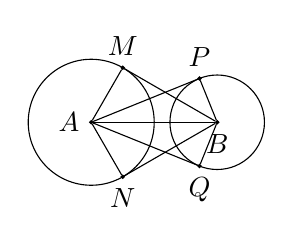
\begin{tikzpicture}[scale =0.2,>=stealth,point/.style = {draw, circle, fill = black, inner sep = 0.4pt},]
\draw (0,0)circle (4cm);
\draw (8,0)circle (3cm);
\node (A) at (0,0)[point,label=left :$A$] {};
\node (B) at (8,0)[point,label=below :$B$] {};
\node (P) at (6.875,2.781)[point,label=above :$P$] {};
\node (Q) at (6.875,-2.781)[point,label=below :${Q}$] {};
\node (M) at (2,3.464)[point,label=above :$M$]{};
\node (N) at (2,-3.464)[point,label=below :${N}$] {};

\draw (A)--(B);
\draw (A)--(M);
\draw (A)--(N);
\draw (B)--(P);
\draw (B)--(Q);
\draw (B)--(M);
\draw (B)--(N);
\draw (A)--(P);
\draw (A)--(Q);
\end{tikzpicture}
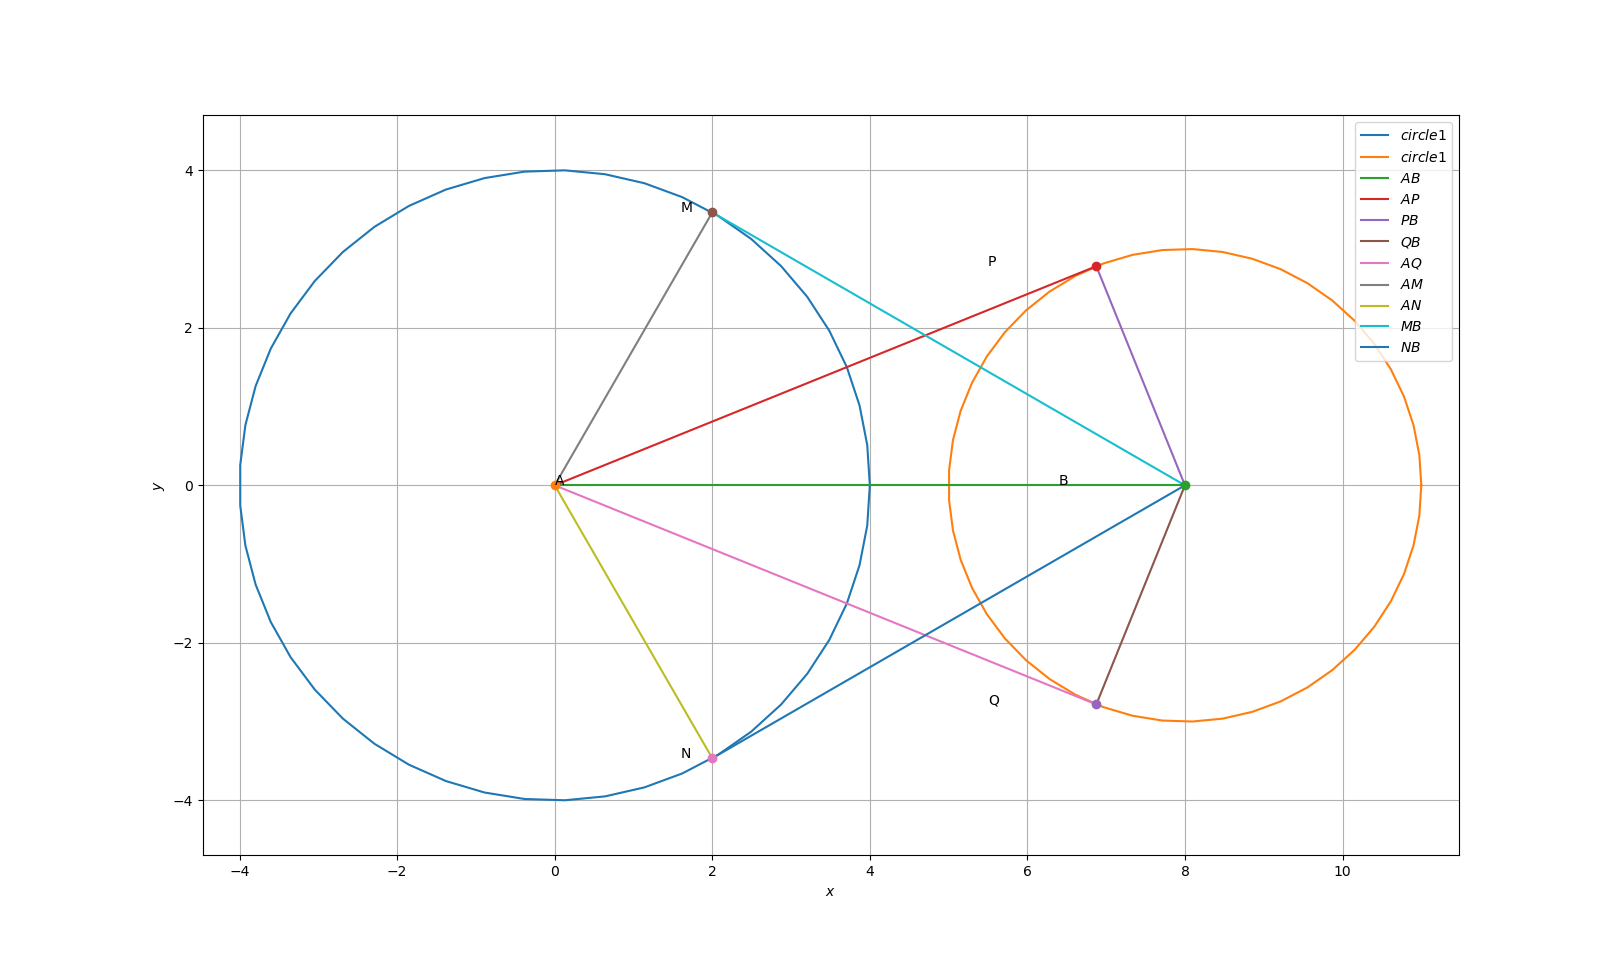
\includegraphics[scale=0.1]{./figs/circon.png}
\end{figure}
\end{frame}